\section{Aufbau der Datenstruktur}
An dieser Stelle der Bachelorarbeit sollen die grundlegenden Eigenschaften der verwendeten Wetterstation dargestellt werden. Eine gute Kenntnis der Datenstruktur sowie der Datenbereitstellung sind eine zwingende Voraussetzung für den späteren Aufbau der MATLAB Funktion. Die nachfolgenden Angaben in diesem Kapitel können der Hardware Spezifikation entnommen werden \cite{HWKDoc} Der Hersteller bietet für die Hardware eine Reihe von Lizenzmodellen an, die den Empfang der Datenmenge bestimmt. Das in dieser Arbeit zum Einsatz kommende Modell nennt sich "{}WS-K RTU485 WPAia T"{} und beinhaltet das Prognosepaket "Premium All inclusive advanced", welches es ermöglicht, das komplette Spektrum an Prognosedaten abzurufen. Welche Wetterinformationen genau zur Verfügung stehen, kann der unten aufgeführten Grafik entnommen werden.
\begin{figure}[h]
\centering
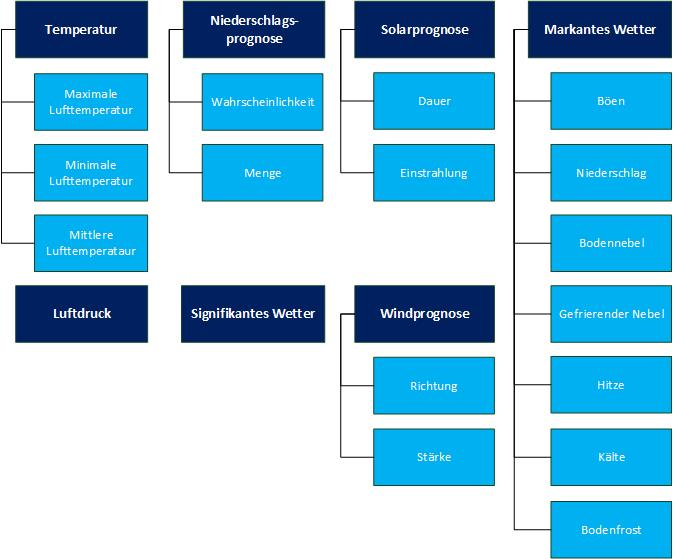
\includegraphics[scale=0.65]{weatherstation/Datenuebersicht}
\caption{Verfuegbare Prognosedaten WS-K RTU485 WPAia}
\label{fig:1}
\end{figure}
Für welche Bereiche diese metereologischen Daten zutreffen muss in der Wetterregion spezifiziert werden. Hier besteht die Möglichkeit für über 1000 Städte in fast ganz Europa die Wetterprognosen abzufragen \cite[S. 27-38]{HKWDoc}. Wie schon in der Einleitung erwähnt, wäre eine niedrige zeitliche Auflösung der Daten wünschenswert, damit das Energiemanagementsystem ohne große Verwerfungen planen kann. Jedoch liegen die meisten Daten in einer Auflösung von 6 Stunden vor, d.h. für ein Intervall von morgens, mittags, nachmittags und abends. Lediglich die mittlere Lufttemperatur wird in einer 1 stündigen Auflösung bereitgestellt. Dieser Umstand wird später im Programmablauf gesondert berücksichtigt. Ein Update der Daten erfolgt ebenfalls alle 6 Stunden. Neben der Auflösung unterscheidet sich auch der Prognosehorizont innerhalb der zugänglichen Daten. Die Spanne reicht von einem bis zu drei Folgetagen. Für den aktuellen Tag, liegen für alle Bereiche Daten vor. Welche metereologische Ausprägung welche Eigenschaften besitzt, kann in der Tabelle \textbf{\ref{tab:detaildatenstruktur}} im Anhang nachvollzogen werden.    
\section{Technischer Aufbau der Station}
\subsection{Senderauswahl und Stationsaufbau}
Die eingesetzte Wetterstation erhält ihre Daten via Langwelle von drei auswählbaren Sendern:
\begin{itemize}
\item Sender Mainflingen DCF 49
\item Sender Burg DCF 39
\item Sender Lakihegy HGA 22 (Ungarn)
\end{itemize}
\begin{figure}[h]
\centering
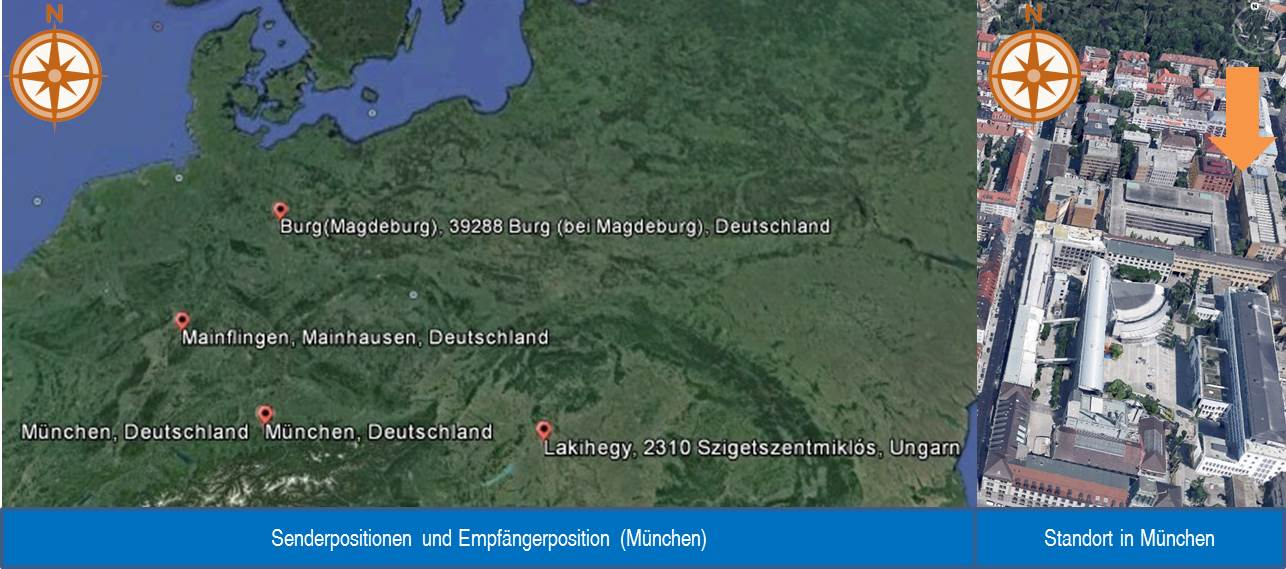
\includegraphics[scale=0.65]{weatherstation/Empfaengerausrichtung}
\caption{Standorte der Langwellensender und des Empfängers}
\label{fig:3}
\end{figure}
Die Wetterstation soll in München aufgebaut werden. Um einen guten Empfang gewährleisten zu können, muss sie entsprechend ausgerichtet werden. Der Hersteller gibt hierzu Kriterien vor, die beachtet werden sollten:
\begin{itemize}
\item senkrechter Aufbau des Gehäuses mit nach unten austretendem Kabelstrang
\item für einen Innenaufbau in der Nähe zum Fenster
\item Mindestabstand von 30 cm zu Metallkonstruktionen oder -flächen
\item ausreichende Entfernung zu Geräten die elektromagnetisch abstrahlen
\item keine direkte Sonnenbestrahlung für das Einbinden der lokalen Temperatur
\item ausreichender Bodenabstand, um Einschneien zu vermeiden
\item Ausrichtung zum geografisch günstigsten Sender
\end{itemize} 
Unter Berücksichtigung dieser Empfehlungen wurde die Station in Fensternähe in nordwestlicher Richtung aufgebaut und die Sendestation Mainflingen vorgegeben.
\subsection{Registereinteilung und Schnittstellenparametrierung}
Wie im vorigen Kapitel bereits erläutert, können über das MODBUS Protokoll vier Arten von Registern angesprochen werden. In der Wetterstation sind zwei Register für die Kommunikation vorgesehen. Im Holdingregister können Einstellungsparameter gesetzt und gelesen werden.\label{comsetreg} Eine Übersicht gibt die oben aufgeführte Tabelle \textbf{\ref{tab:kommeinstpara}}.
\begin{table}[t]
\caption{Einstellungsparameter für den Kommunikationsaufbau und den Wetterbereich}
\rowcolors{1}{cyan}{white}
{
\setlength{\extrarowheight}{0.1cm}
\begin{tabular}{| c | l | c | l | l | p{2.5cm} |}
\hline
\textbf{\parbox[t]{1.8cm}{Register-\\adresse}} & \textbf{Bezug} & \textbf{Zugriff} & \textbf{Datentyp} & \textbf{Bereich} & \textbf{Bemerkung}\\[1cm]
\hline \hline
\hiderowcolors
110 & Senderstation & Lesen/Schreiben & unsigned & 0,1,2 & 0 = DCF 49 \newline 1 = HGA 22 \newline 2 = DCF 39\\
111 & Empfangsqualität & Lesen & unsigned & 0...9 & 9 ist höchste Qualität\\
112 & Stadt ID & Lesen/Schreiben & unsigned & 0...1022 & \\
100 & Sekunde (Funkuhr) & Lesen & unsigned & & UTC\\ 
101 & Minute (Funkuhr) & Lesen & unsigned & & UTC\\
102 & Stunde (Funkuhr) & Lesen & unsigned & & UTC\\
103 & Tag (Funkuhr) & Lesen & unsigned & & UTC\\
104 & Monat (Funkuhr) & Lesen & unsigned & & UTC\\
105 & Jahr (Funkuhr) & Lesen & unsigned & & UTC\\
\hline
\end{tabular}
}
\label{tab:kommeinstpara}
\end{table} 
Außerdem sind sämtliche metereologischen Daten in diesem Register abgelegt. Eine Auflistung der den Prognosebereichen zugeordneten Registeradressen gibt die im Anhang befindliche Tabelle \ref{tab:detaildatenstruktur}. Es ist dabei zu beachten, dass die Adressen gegenüber den in der Spezifikation des Herstellers Angegebenen, bereits auf die Struktur des Holdingregisters angepasst wurden. D.h. da das Holdingregister mit einer 0 beginnt, wurde von jeder Adresse eine Position abgezogen. Neben dem Holdingregister gibt es noch das Coilregister, in welchem die Zustände für den externen Temperatursensor und die FSK Qualität vorgehalten werden. Die Adressen hierfür sind 1 bzw. 2 und die zugelassenen Werte 1 und 0 geben jeweils den Zustand an. 1 bedeutet der Sensor sowie die FSK Qualität sind in Ordnung.\label{coilabfrage} 
\begin{wraptable}{r}[0mm]{35mm}
\caption{Schnittstellenparameterbelegung}
\rowcolors{1}{cyan}{white}
{
    \begin{tabular}{| l | c |}
    \hline
    	\textbf{Parameter} & \textbf{Wert}\\ \hline
\hiderowcolors 
      	Baudrate & 19600 \\ \hline
      	Parität & even \\ \hline
      	Databit & 8 \\ \hline
      	Stopbit & 1 \\ \hline
      	Slave-Adresse & 03 \\ \hline
    \end{tabular}
    \label{tab:parabel}
}
\end{wraptable}
Um eine funktionierende MODBUS Kommunikation über eine serielle Schnittstelle aufbauen zu können, müssen bestimmte Schnittstellenparameter beim Empfänger sowie beim Sender identisch sein. Die Baudrate gibt dabei an, wieviele Bits pro Zeiteinheit übertragen werden können \cite[S .169]{Kuveler.2007}. Das Paritätsbit zeigt an, ob im übertragenen Byte ein 1 bit Fehler vorliegt. Dies ist dann der Fall, wenn die Zahl der übertragenen Einsen ungerade ist, jedoch das Paritätsbit (= 0 bei even und 1 bei odd) eine gerade Anzahl anzeigt. Das Kommunikationprotokol erfordert in diesem Fall eine erneute Übertragung der Information \cite[S. 25]{Kuveler.2007}. Das Databit gibt lediglich die Anzahl der zu übertragenden bits pro Codewort an. Das Stopbit, entweder 1 oder 2 bits, wird zur Synchronisierung von Sender und Empfänger benötigt, damit diese wissen, wann ein Codewort beginnt und endet \cite[S. 169-170]{Kuveler.2007}. Per Jumperpositionierung kann die Baudrate von 9600 auf 19200 in der Wetterstation geändert werden, die Werkseinstellung von 19200 wurde aber in dieser Arbeit beibelassen. Ebenso einstellbar über Jumper ist die Slave-Adresse der Wetterstation. Aber auch hier wurde der voreinstellte Wert nicht verändert. Nachdem nun das Modbusprotokoll und die Funktionsweise der Wetterstation bekannt sind, kann mit der Umsetzung der MATLAB Funktion begonnen werden.     


    
